\section{Variables}
\subsection{Independent Variables and Dependent Variables}
The independent variable for this experiment is the temperature of the solution, which is measured by a Vernier Temperature Probe with a precision of $\pm 0.1^\circ C$. The dependent variable for my experiment is the absorbance of a monochromatic light source of the thiocyanatoiron(III) complex ion in the reaction, which is measured using a spectrophotometer with a precision of $\pm 0.00035$ transmittance. The transmittance will be used to derive the concentration of the thiocyanatoiron(III) complex ion and thus the equilibrium constant of the reaction. More details about the specific measurement processes are described in the \cref{section:procedure}.

\subsection{Control Variables}
I ensured that all other variables were controlled to get accurate results about the relationship between the equilibrium constant and temperature. For example, throughout the trials, the solution remained untouched so that no variations would occur due to the slight variations in the initial concentrations of \(Fe^{3+}\) and \(SCN^-\). Furthermore, the same amount of water (200 mL) at roughly the same initial temperature ($<20^\circ C$) was used for every trial with the same heating source to ensure that the controlled temperature increased at the same rate throughout the trials. Finally, the beaker, temperature probe, and thermistor were always cooled down to room temperature before proceeding to do a new trial. Through all measures, a more accurate relationship between my independent and dependent variables can be assessed.

\section{Methodology}
\subsection{Materials}
\begin{itemize}[noitemsep,nolistsep]
    \item Vernier Temperature Probe, $\pm 0.1^\circ C$
    \item GoLink (for connecting to Logger Pro)
    \item Logger Pro Software on Laptop (for dynamic temperature logging)
    \item Spectrophotometer (for use in colorimetry), $\pm 0.01 \%$ 
    \item 1.2 cm Square Cuvettes (to hold spectrophotometer sample)
    \item Hot Plate (as heat source)
    \item 400 mL Glass Beaker
    \item Beaker Tongs and Wire Gauze (to handle hot beaker)
    \item Forceps (to move hot cuvettes)
    \item $Fe(NO_3)_3$ Solution, $0.100 \; M$
    \item $KSCN$ Solution, $0.001 \; M$
    \item $Fe(NO_3)_3$ Solution, $0.025 \; M$
    \item $KSCN$ Solution, $0.025 \; M$
    \item Deionized Water
\end{itemize}

% \subsection{Experimental Setup}
% \begin{figure}[ht]
%     \centering
%     \includegraphics[width=\textwidth,height=100mm,keepaspectratio]{images/IA_Schematic.png}
%     \caption{Schematic for Chemistry IA Experiment Setup}
%     \label{fig:schematic}
% \end{figure}


% \begin{figure}[H]
%     \centering
%     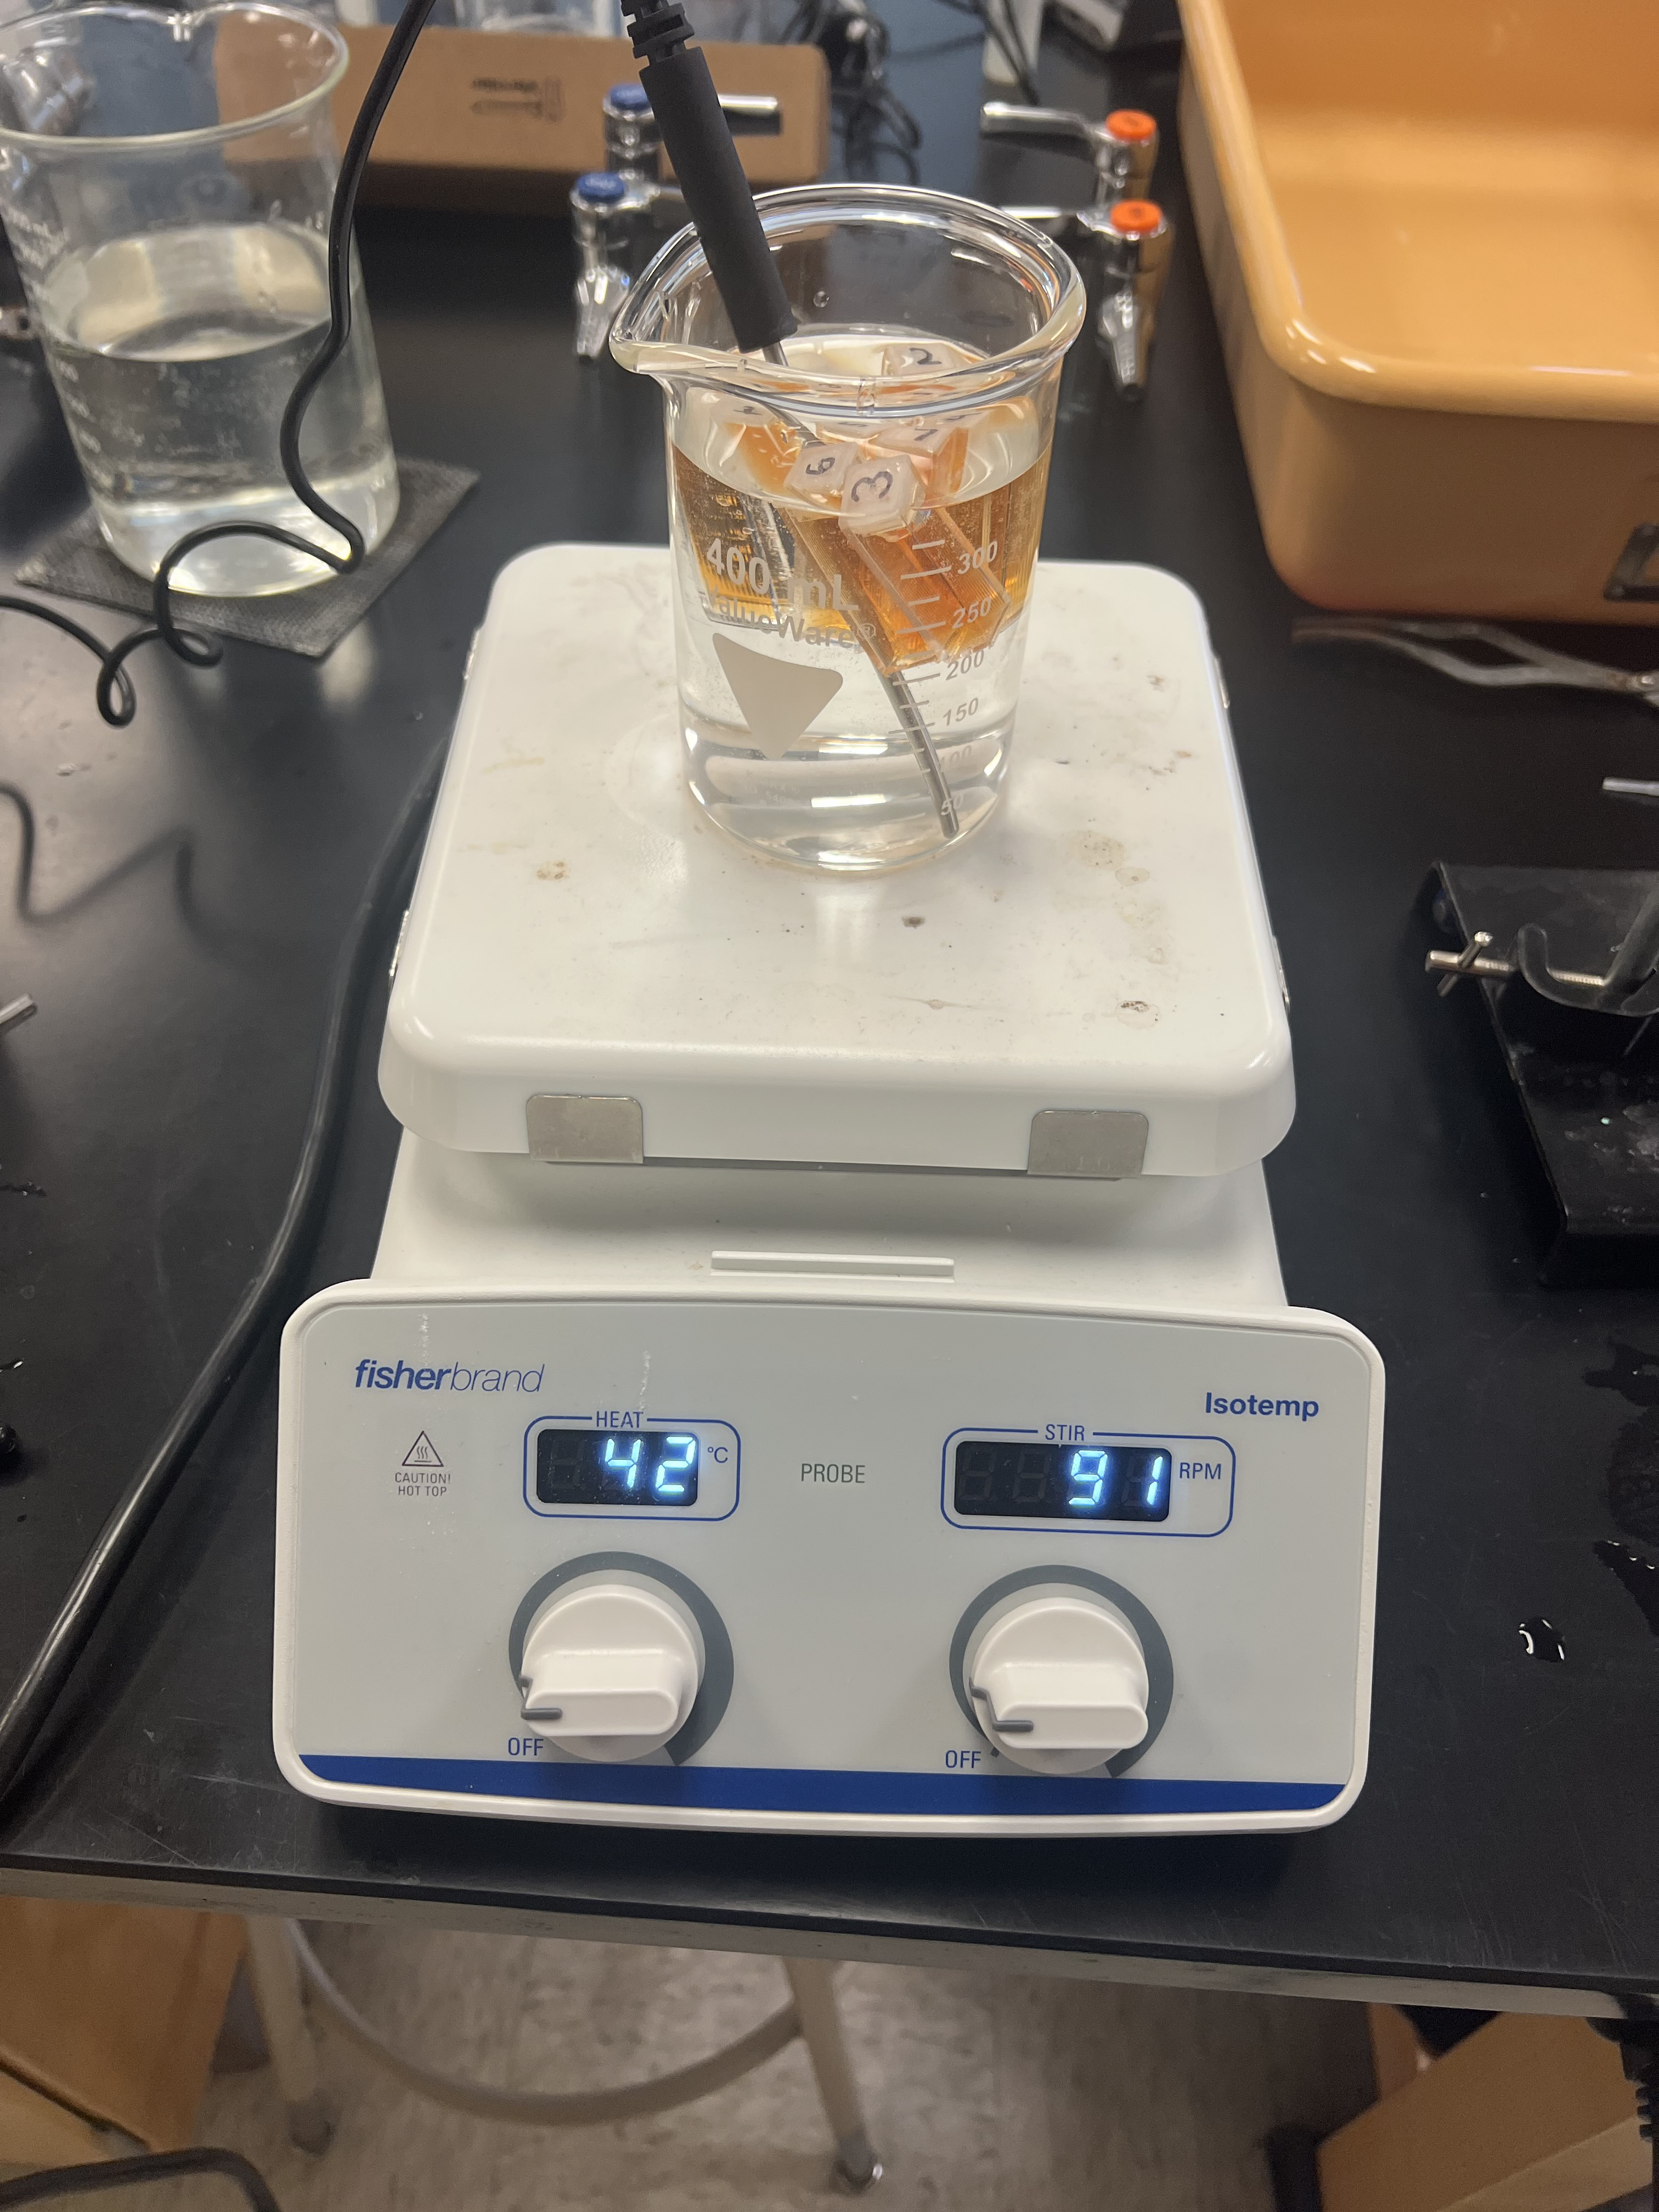
\includegraphics[width=50mm,height=\textheight,keepaspectratio]{images/setup.png}
%     \caption{Example Experimental Setup}
%     \label{fig:setup}
% \end{figure}

\section{Procedure}
\label{section:procedure}
Create a blank DI water sample for spectrophotometer calibration. Create the standardization samples as per \cref{table:procedure} and fill a cuvette with each. Record the transmittance for each standardization sample.

\begin{table}[H]
\centering
\begin{tabular}{|C{3cm}|C{4cm}|C{4cm}|}
\hline
Volume of 0.1M \(Fe(NO_3)_3\) (\(mL\)) & Volume of 0.001M \(KSCN\) (\(mL\)) & Volume of Deionized Water (\(mL\)) \\ \hline
2.00         & 5.00        & 5.00            \\ \hline
3.00         & 4.00        & 5.00            \\ \hline
4.00         & 3.00        & 5.00            \\ \hline
5.00         & 2.00        & 5.00            \\ \hline
6.00         & 1.00        & 5.00            \\ \hline
\end{tabular}
\caption{Spectrophotometer Standardization Samples}
\label{table:procedure}
\end{table}

Next, prepare a 45 mL solution in a beaker using 3 mL of \(Fe(NO_3)_3\) (0.025 M), 3 mL of \(KSCN\) (0.025 M), and 39 mL of DI water. Pipette this solution into 7 separate cuvettes. Place the cuvettes in a 300 mL water bath inside glass beaker.

Setup and calibrate spectrophotometer using blank sample before running the experiment, so heat dissipated from the sample is minimized. Plug Vernier Temperature Probe into the laptop via the GoLink to log the temperature readings. Open up Logger Pro software to get live temperature readings. 

Place the beaker on the hot plate and turn on the heating. Perform the following steps for 10 different temperature levels starting at 25 degrees and increasing by 5 degrees. First, use the temperature probe to determine when the sample is at the desired temperature. Wait approximately 2-3 minutes to ensure cuvettes reach same temperature as hot water bath. Pick up one cuvette using forceps and wipe off any surface water with Kimwipes. Measure the transmittance using the spectrophotometer to determine the unknown equilibrium concentrations and thus the \(K_c\). Return the cuvette back to water bath and select another cuvette for a total of 14 trials. Repeat this whole process for the remaining temperature levels.

\section{Safety, Environmental, and Ethical Concerns}
Throughout this investigation, all safety, environmental, and ethical concerns were recognized and thoroughly addressed. First, the major hazard in this lab is the heating source. Thus, multiple solutions were implemented to mitigate risks. The experiment was approved and performed under teacher supervision using proper experiment apparatus such as wire gauze and beaker tongs. The glass beaker was also cooled slowly to ensure that it would not shatter upon a rapid temperature change. All these measures greatly improved safety, leading to no injuries during the course of the experiment. Second, the thiocyanatoiron(III) complex reaction utilized is relatively harmless. Still, since \(Fe(NO_3)_3\) is a body tissue irritant and \(KSCN\) is harmful if swallowed, in contact with skin, or inhaled, I conducted the experiment wearing safety glasses and nitrile gloves in an environment with open circulation. Third, there were no environmental concerns as a significant amount of natural resources were not utilized and pollution was not generated. Finally, there were no ethical concerns as no humans, animals, or other beings were physically or emotionally harmed in this experiment.